\documentclass[article, onecolumn, ,nofootinbib,nopreprintnumbers]{revtex4}


%%%%% AUTHORS - PLACE YOUR OWN MACROS HERE %%%%%
\usepackage{epsfig}
\usepackage{graphicx}
\usepackage{color}
\usepackage{ulem}
%%\usepackage{nopageno}
%%\usepackage{txfonts} % this one creates conflict
%\usepackage[usenames]{color}
\usepackage{endnotes}
%\usepackage[authoryear]{natbib}

%%\usepackage{latexsym}
%%\usepackage{moreverb,longtable,subfigure}
\usepackage{amssymb}
\usepackage{amsmath,bm}
\usepackage{times}
\usepackage{subfigure}
%\usepackage{aas_macros}
\usepackage{verbatim}

\newcommand{\be}{\begin{equation}}
\newcommand{\ee}{\end{equation}}
\newcommand{\bdm}{\begin{displaymath}}
\newcommand{\edm}{\end{displaymath}}
\newcommand{\bea}{\begin{eqnarray}}
\newcommand{\eea}{\end{eqnarray}}

\newcommand{\apjl}{Astrophysical Journal, Letters}
\newcommand{\mnras}{MNRAS}
%\newcommand{\prd}{Phys. Rev. D}
%\newcommand{\apj}{Astrophysical Journal}
\newcommand{\aap}{Astronomy and Astrophysics}
\newcommand{\sovast}{Soviet Ast.}
%\newcommand{\nat}{Nature}

\newcommand{\cm}{\textcolor{magenta}}

\newcommand{\cf}{\textit{cf.}~}
\newcommand{\ie}{\textit{i.e.}~}
\newcommand{\eg}{\textit{e.g.}~}
\newcommand{\mss}{{\rm ms}}
\newcommand{\km}{{\rm km}}
\newcommand{\hz}{{\rm Hz}}
\newcommand{\khz}{{\rm kHz}}
\newcommand{\mpc}{{\rm  Mpc}}
\newcommand{\Msolar}{\ensuremath{\Msun}}
\newcommand{\mc}[1]{\textcolor{green}   {\texttt{\textbf{MC: #1}}} }
\newcommand{\md}[1]{\textcolor{blue}   {\texttt{\textbf{MD: #1}}} }
\newcommand{\jc}[1]{\textcolor{red}    {\texttt{\textbf{JC: #1}}} }
\newcommand{\stanny}[1]{\textcolor{cyan}   {\texttt{\textbf{CR: #1}}} }
\newcommand{\sesa}[1]{\textcolor{magenta}   {\texttt{\textbf{SESA: #1}}} }

\newcommand{\mtrx}[1]{\bm{#1}}

\newcommand{\msun}{M_\odot}
\def\lsim{\lower.5ex\hbox{$\; \buildrel < \over \sim \;$}}

\newcommand{\incgraph}[3]{\includegraphics[angle=#1, width=#2\textwidth]{#3}}


%%%%%%%%%%%%%%%%%%%%%%%%%%%%%%%%%%%%%%%%%%%%%%%%
\begin{document}

%\title{European Pulsar Timing Array constraints on anisotropy in the nanohertz stochastic gravitational-wave background}
\title{Friday practicum: stochastic gravitational wave backgrounds}
\author{Chiara M. F. Mingarelli}
\affiliation{TAPIR (Theoretical Astrophysics), California Institute of Technology MC 350-17, Pasadena, California 91125, USA}
\author{Michele Vallisneri}
\affiliation{TAPIR (Theoretical Astrophysics), California Institute of Technology MC 350-17, Pasadena, California 91125, USA}
\affiliation{Jet Propulsion Laboratory, California Institute of Technology, Pasadena, California 91109, USA}
\author{Yanbei Chen}
\affiliation{TAPIR (Theoretical Astrophysics), California Institute of Technology MC 350-17, Pasadena, California 91125, USA}

\date\today
\maketitle

\section{Introduction}
In today's lectures, you have explored Testing General Relativity with GW observations, \cm{[Michele add a blurb about your lectures]}, and how to detect low frequency GWs using Pulsar Timing Arrays. The following exercises are meant to cement these concepts. These come in at least 2 flavors: general exercises, and advanced ones for those who may already be familiar with these concepts and are up for a challenge! 

\section{Exercises}
Do as many of the following exercises as time allows. If you get stuck, please ask a Lecturer or a teaching assistant for help.

\subsection{Pulsar Timing Arrays}
Pulsar timing arrays are sensitive to GWs in the nanoHertz frequency regime. Sources here include supermassive black hole binaries, primordial (or relic) GWs from inflation, and cosmic strings. The goal of this exercise is to derive the overlap reduction function for an isotropic stochastic GW background. This is often referred to as the Hellings and Downs curve \cite{HellingsDowns:1983}.

 %

\begin{figure}[b]
		\centering
		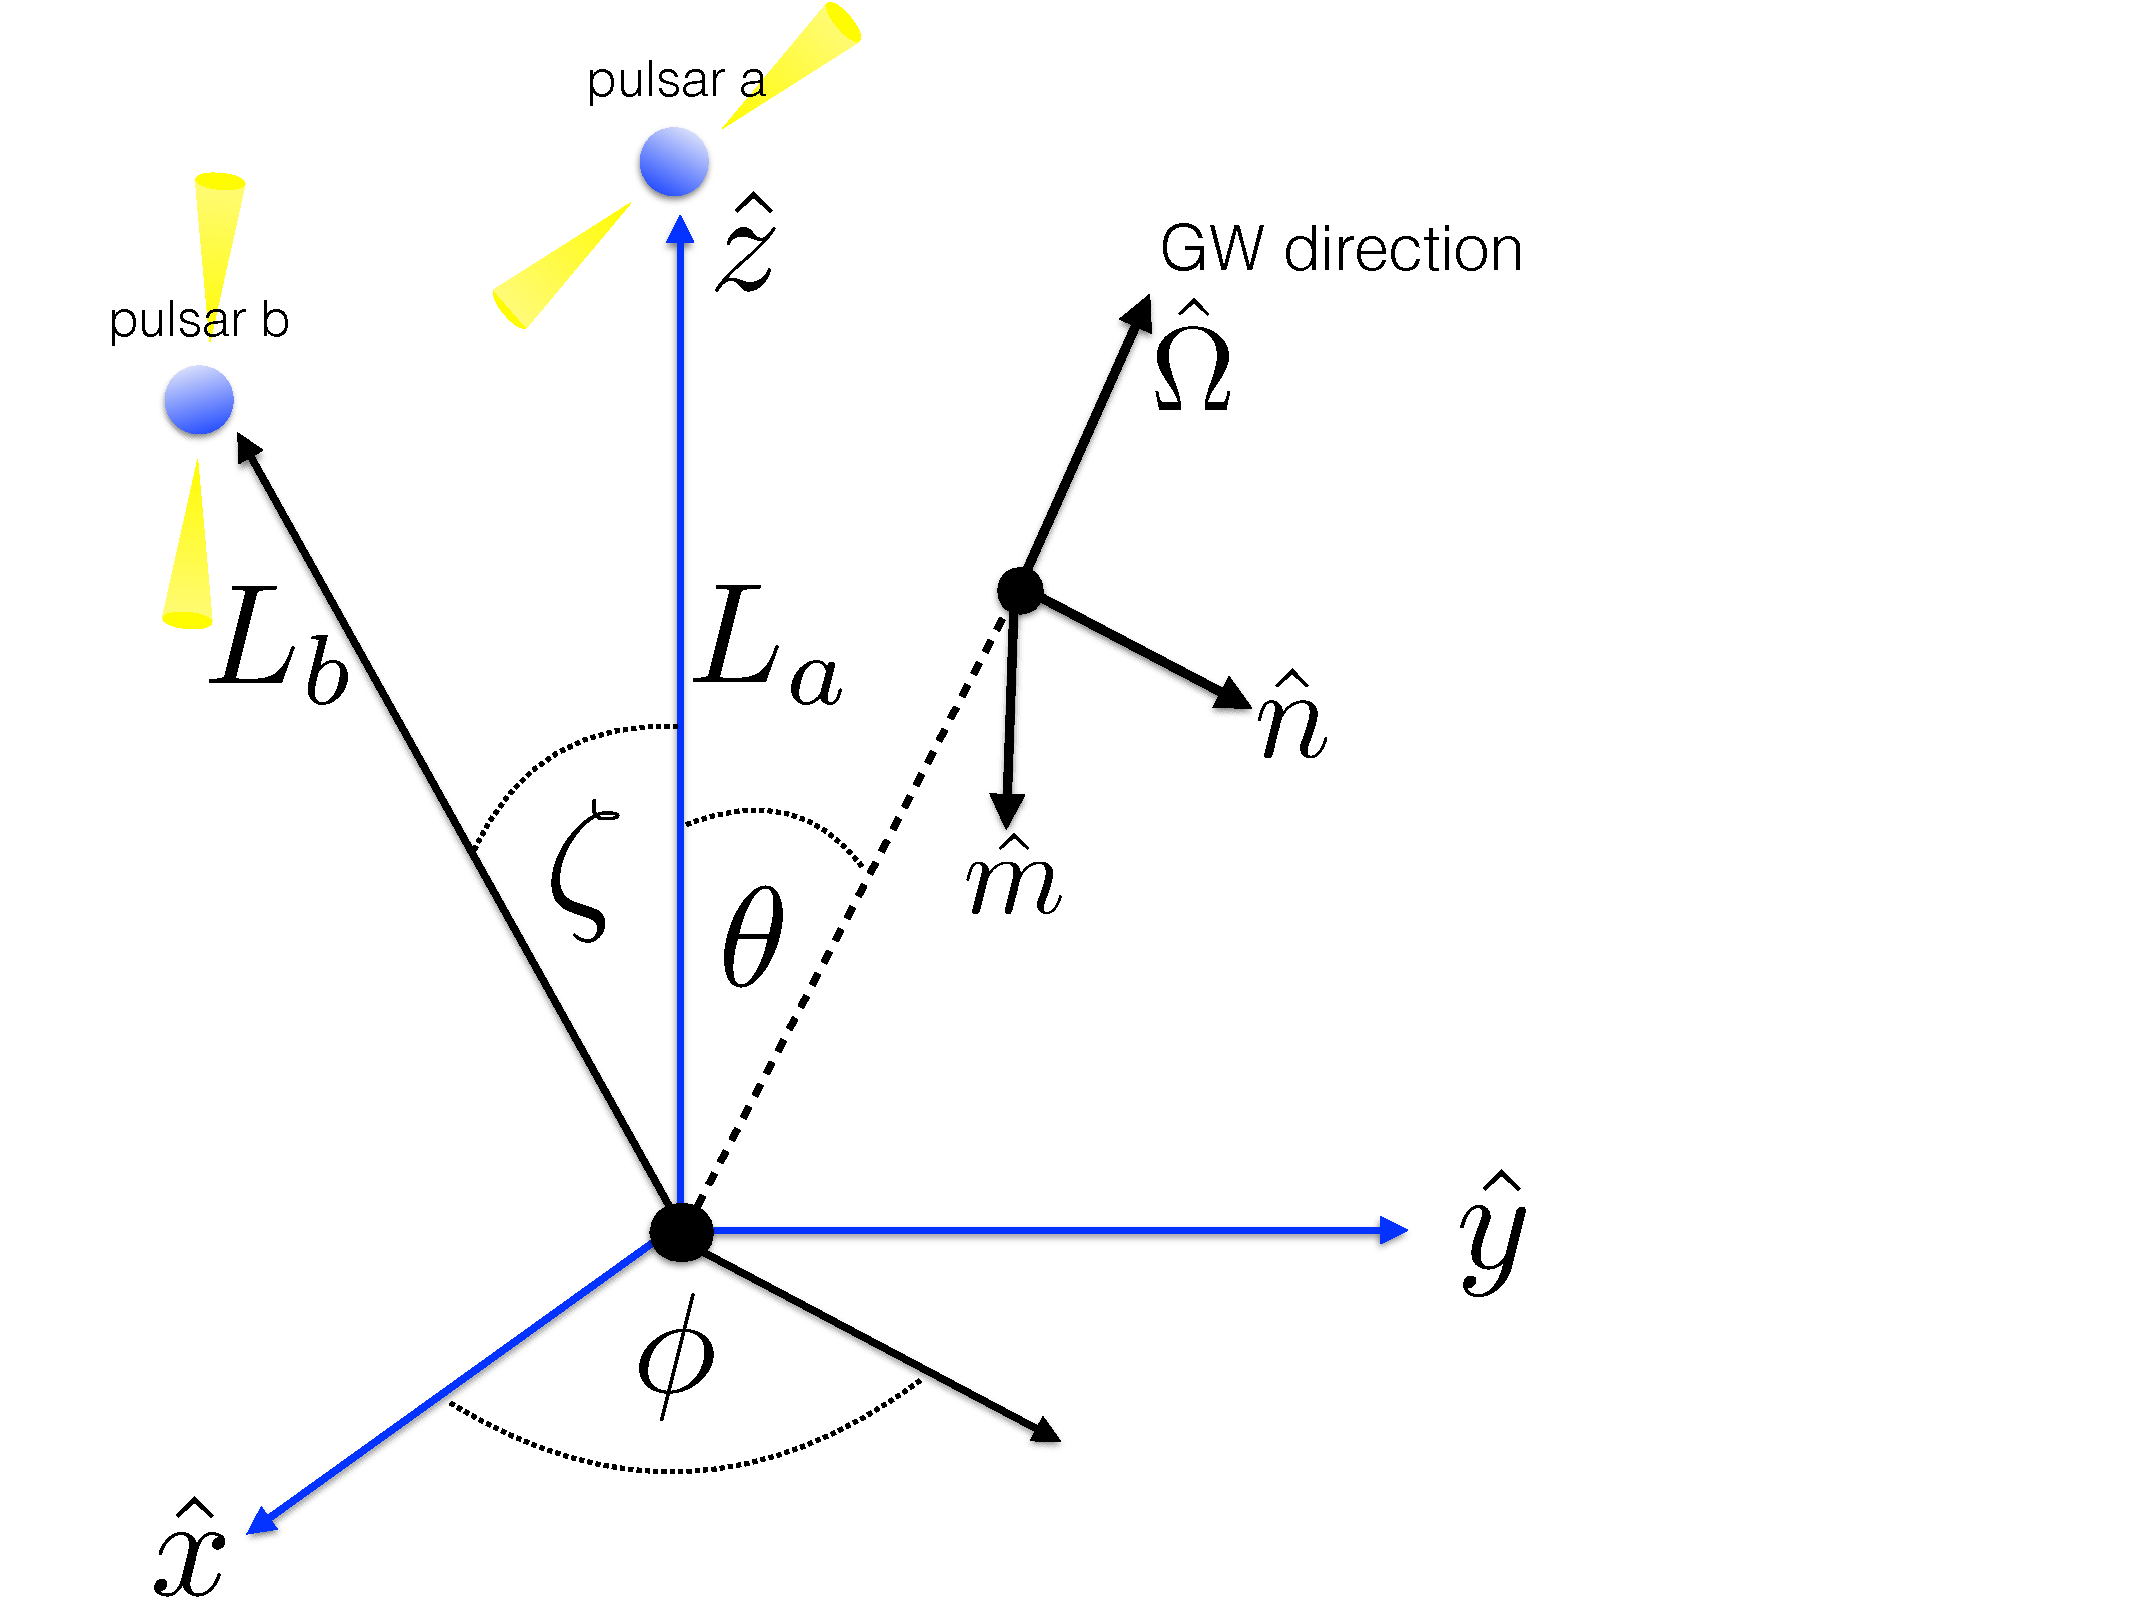
\includegraphics[width=3.9in]{pta_geometry.pdf}
		\caption[Typical pulsar timing array geometry]{Suggested geometry: pulsar $a$ is on the $z$-axis at a distance $L_a$ from the origin (solar system barycentre), pulsar $b$ is in the $x$-$z$ plane at a distance $L_b$ from the origin making an angle $\zeta$ with pulsar $a$. $\hat\Omega$ is the direction of GW propagation with principal axes $\hat m$ and $\hat n$ such that  $\hat m \times \hat n =\hat\Omega$. The polar and azimuthal angles are given by $\theta$ and $\phi$, respectively.}
		\label{fig:geometry}
	\end{figure}


\begin{enumerate}
\item For a pair of pulsars $a$ and $b$, define a reference frame. Specifically, write down the unit vectors which point to the pulsars, $\hat{p}_a$, $\hat{p}_b$, the direction of GW propagation $\hat{\Omega}$ and the principal axes $\hat m$, $\hat n$, such that $\hat m\times \hat n = \hat \Omega$.  {\it Hint, place pulsar $a$ on the z-axis and $b$ in the x-z plane}

\item Write down the general expression for the antenna beam pattern, 
\begin{equation}
F^A(\hat \Omega) = \frac{1}{2} \frac{\hat p^i \hat p^j}{1+\hat\Omega\cdot\hat p} e^A_{ij}(\hat\Omega) \, ,  
\end{equation}
where $A=+,\times$ is the GW polarization. The polarization tensors $e^+_{ij}(\hat \Omega) = \hat m_i\hat m_j - \hat n_i \hat n_j$, $e^\times_{ij} (\hat \Omega)= \hat m_i \hat n_j + \hat n_i \hat m_j$. For further reading, see \cite{AllenRomano:1999, Anholm:09}. 


\item Give expressions for $F^+_a$, $F^\times_a$, $F^+_b$, $F^\times_b$ in your chosen coordinate frame
\item The overlap reduction function is given by integrating the antenna beam patterns over the sky, i.e. over all possible GW directions $\hat \Omega$:
\begin{equation}
^{(ab)}\Gamma(\zeta)=\int_0^\pi  \sin\theta d\theta \int_0^{2\pi} d\phi  \sum_A F^A_a(\hat \Omega) F^A_b(\hat \Omega) \, ,
\end{equation}
where $\zeta \in [0,\pi] $ is the angle between the pulsars. Using your expressions for the antenna beam pattern, you may either integrate the above expression analytically (hint, use contour integration) or open the ipython notebook and do this numerically. Plot the result for all $\zeta$. The result is the Hellings and Downs curve! 

\item Which of these steps implicitly assumes an isotropic background? Where would we modify this calculation to take in to account anisotropy in the GW background? More on this in \cite{MingarelliEtAl:2013}.
\end{enumerate}



\subsection{Testing GR}

Having built the above tools, Let us move on to explore testing GR in the context of GW background in PTAs.  We will do this in two steps: first, we shall compute the overlap reduction function in more general theories of gravity.  
\begin{enumerate}
\setcounter{enumi}{5}
\item Suppose GW has a scalar component, i.e., for a gravitational wave propagating along the $\hat\Omega$ direction, we have 
\begin{equation}
e^{\circ}_{ij}(\Omega)=\hat m_i\hat m_j+\hat n_i \hat n_j\,.
\end{equation}
Write down the antenna beam pattern and compute the overlap reduction function.  
\item Suppose, {\it instead}, that the graviton is actually massive, and that the GW has a dispersion relation 
\begin{equation}
\omega^2 = m_g^2 +k^2\,.
\end{equation}
In other words, a single-frequency plane GW produces the following metric perturbation: 
\begin{equation}
h_{ij} (t,\mathbf{x}) = e^{-i\omega(k) t+ i k\hat\Omega\cdot\mathbf{x}} \left[
H_+ e^{+}_{ij} +
H_\times e^{\times}_{ij}\right]
\end{equation}

Write down the antenna beam pattern and the overlap reduction function. 
\end{enumerate}
As a second step, let us explore how to distinguish between a standard GR background and a non-GR background. 
\begin{enumerate}
\setcounter{enumi}{7}
\item Based on our result of the overlap reduction function for a scalar background, can we independently extract the scalar and the tensor background?  
\item In the massive gravity case: if we do detect a stochastic background, can we use it to constrain the graviton mass?  How well can we do so?
\end{enumerate}

\subsection{Cosmology with GWs}

\begin{enumerate}
\setcounter{enumi}{10}

\item Solve the scalar-wave propagation equation $\square \phi(x) = 0$ in the Friedmann--Robertson--Walker spacetime
%
\begin{equation}
ds^2 = -dt^2 + a(t)^2 [dx^2 + dy^2 + dz^2],
\end{equation}
%
and show that it admits solutions in the form
%
\begin{equation}
\phi(r,t) = \frac{1}{r \, a(t_0)} g(t - r/c),
\end{equation}
%
where $r = \sqrt{x^2 + y^2 + z^2}$ and $t_0$ is the time at the present epoch. [Hint: introduce a \emph{conformal time} $\eta$ that satisfies $d \eta = dt / a(t)$, and use the curved-space d'Alembertian $\square = 1/\sqrt{-g} \partial_\mu (\sqrt{-g} g^{\mu \nu} \partial_\nu)$].

\item Solve problem 19.10 from Lightman et al.'s \textit{Problem book in relativity and gravitation} (Princeton, 1975; online at \url{http://www.nrbook.com/relativity}). 

\begin{center}
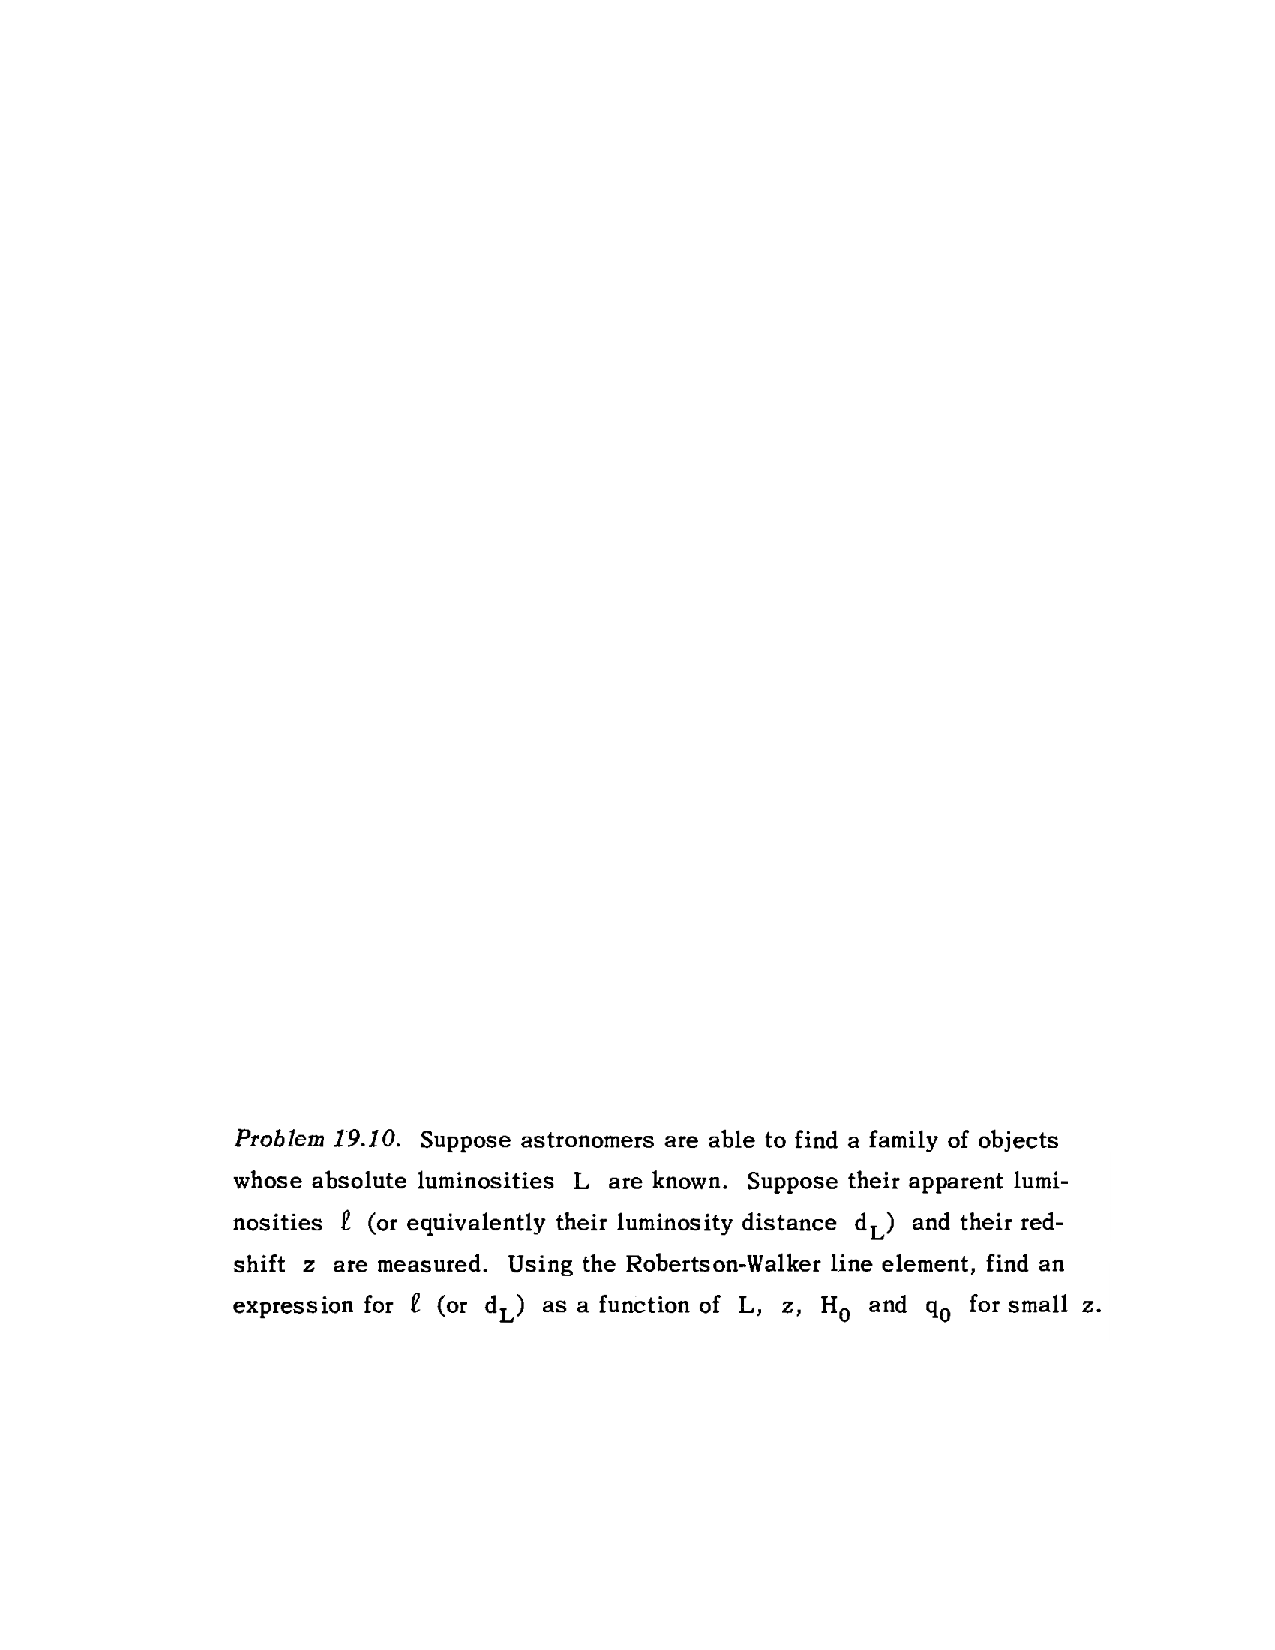
\includegraphics[width=5in]{problem-19-10.pdf}
\end{center}

\end{enumerate}

\bibliography{references}





\end{document}